% ---------------------------------------------------------------------------- %
\begin{figure}
	\centering
	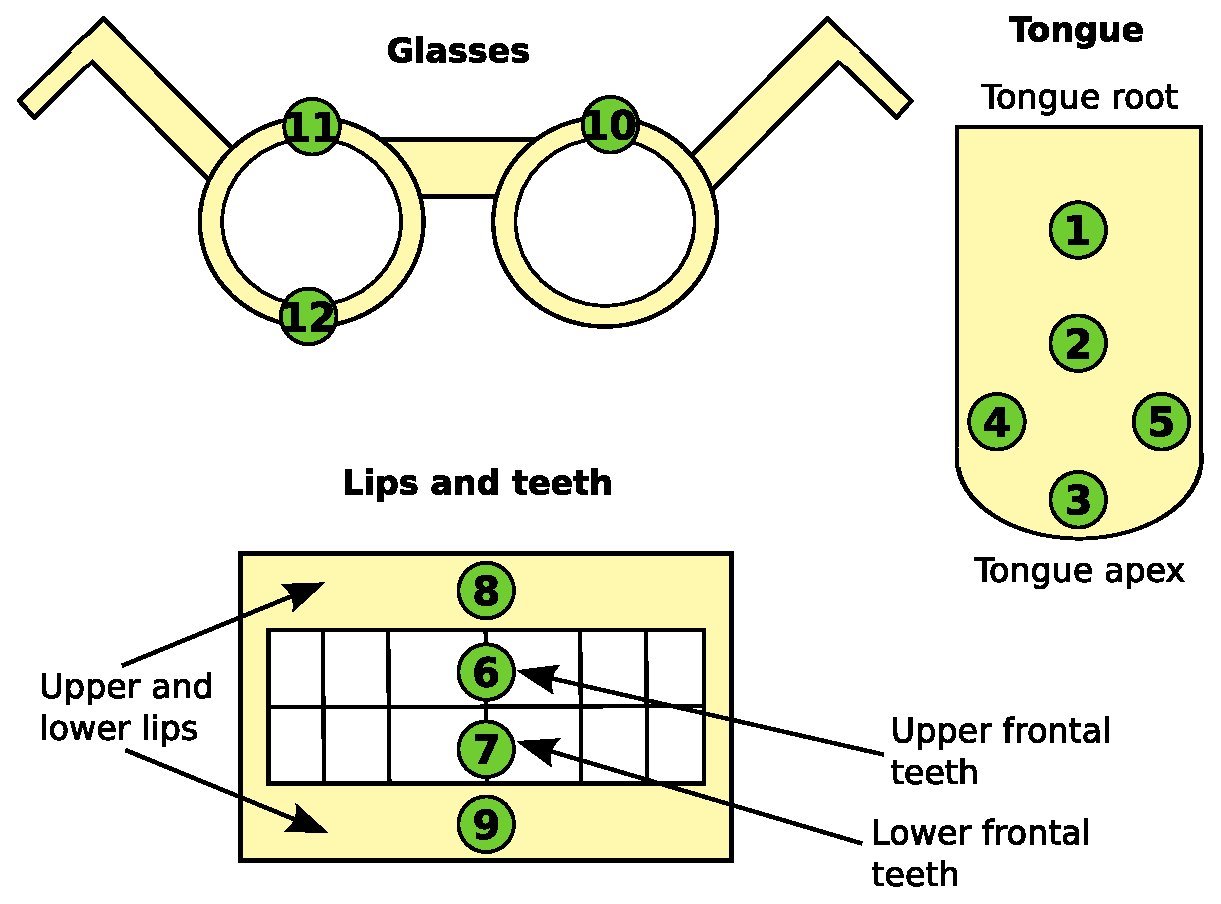
\epsfig{file=include/experiments/images/map.eps, width=0.75\textwidth}
	\caption[Sensor map]{\textbf{Sensor map}:
	in order not to stress the subjects, the experiments never took pictures 
	of the inaccessible sensors. For this reason, the sensor map provides a
	useful representation of the positions of the twelve sensors during
	the Linguometer recordings.
	Note: coronal view of the mouth (\emph{Lips and teeth}) and of the
	\emph{Glasses}; axial view of the \emph{tongue}.}
	\label{fig:experiments:map}
\end{figure}
% ---------------------------------------------------------------------------- %
